\section{Design and the \textit{open-closed-principle}}
One main purpose of the use of java and object-oriented programming is that the code is easily
extended so new features and functions can easily be added to an already working system.
Nevertheless, one has to respect some rules of programming in order to benefit from this
advantage, i.e. the use of design patterns.
In our \textit{MyFoodora} we used several of these patters which are explained in this section.

\subsection{Package Management}
\label{sub:package_management}

Having read the project requirements for the first time we figured out that there were several
different parts which can be treated seperately. This logic sepration of different parts of the
system was used to organize our packages as well as the division of the work for the two members
of the group. The following main packages exist in the project:
\begin{itemize}
	\item{\textbf{system}} Contains the main funtionalities of \textit{MyFoodora}.
	\item{\textbf{user-management}} Manages users of the systems and asseses functions
		to groups of users.
	\item{\textbf{restaurant}} Manages the creation of meals and singleItems and do the
		pricing.
	\item{\textbf{commandLineTool}} Adds a command line user interface to the system.
	\item{\textbf{GUI}} Adds a graphical user interface to the system.
	\item{\textbf{several Test packages}} According their name they provide test for the
		previous packages.
\end{itemize}

The following diagram shows the interaction of the first three packages (The interfaces and
testings do obviously interact with all the other ones).

\begin{figure}[H]
	\centering
	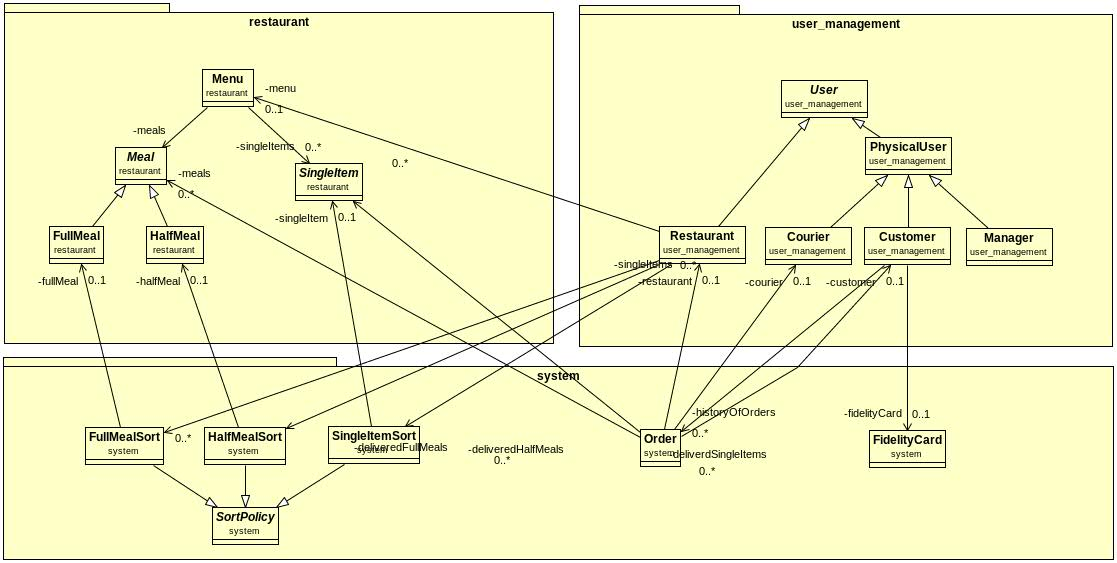
\includegraphics[width=1\linewidth]{./ima/packages.jpg}
	\caption{Package-interactions, class \textit{MyFoodora} excluded to simplify}
	\label{fig:packages}
\end{figure}

The graphic \ref{fig:packages} shows the three main packages that form the core of our system. All
interaction between the packages are displayed except from those with the class
\textit{MyFoodora}. The seperation choosen allowed us to seperately work on the
\textsc{user-management} and \textsc{restaurant} without depending on parts of the code of the
other package, because there is only one interaction between the two. In a third stey we
implemented \textsc{system}, because it was the most sophisticated one and requires large parts of
the two other packages. \textit{Order} is the most connected class besides \textit{MyFoodora}. One
might consider to place it in a of the other packages. We decided to store it in the system
because we wanted functions like the computation of an order's price to be part of the system. In
this manner we were able to keey all the core functions together. 

\subsection{DesignPattern : Factory-Pattern}
\label{sub:designpattern_factory_pattern}

A major pattern to respect the \textit{open-closed-principle} is the Factory-Pattern because it
allows the code to be easily extended without modifying the existing code. It is used twice in
the system:
\begin{enumerate}
	\item Creation of Items for the Restaurant
	\item Creation of Users in the user-management
\end{enumerate}

\paragraph{Creation of Items for the Restaurant}

In order to handle the creation of \textsc{singleItems} and \textsc{meals} in the same method we 
decided to use a \textbf{Factory-Pattern} with an \textit{abstract factory} and a
\textit{factoryProducer}. 

\begin{figure}[H]
	\centering
	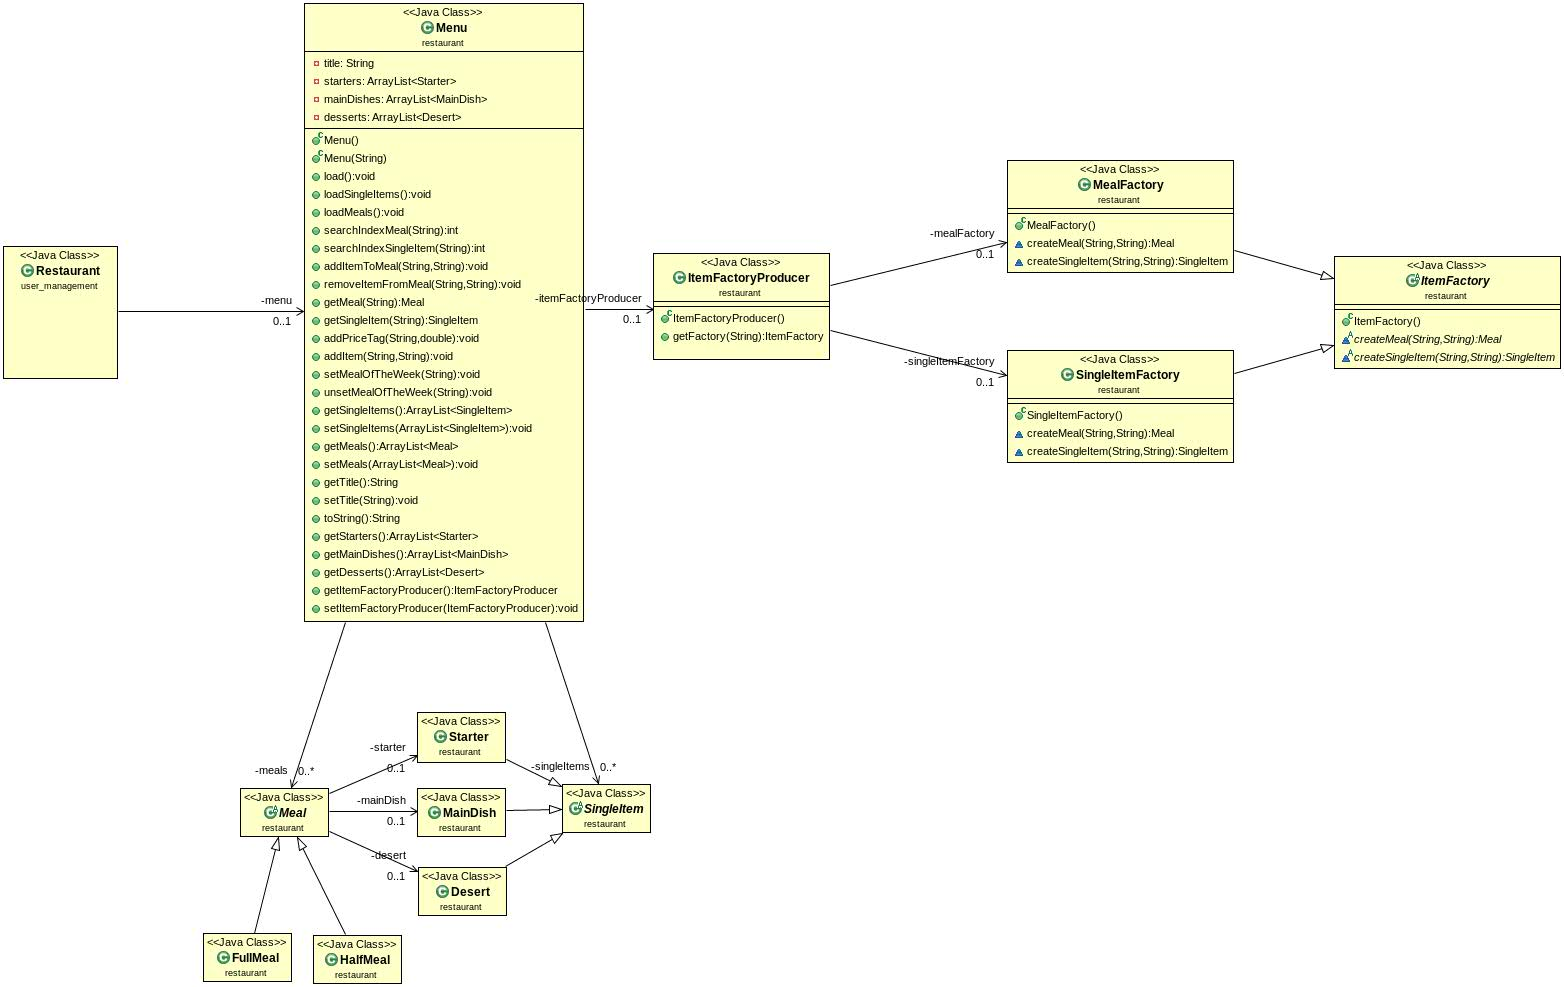
\includegraphics[width=1\linewidth]{./ima/restaurant_factory_pattern.jpg}
	\caption{Factory-Pattern in package \textsc{restaurant}}
	\label{fig:restaurant-factory-pattern}
\end{figure}

The \textsc{Menu} is the center class of \textsc{restaurant} which has an instance of 
\textsc{ItemFactoryProducer} to produce new items and store them in an ArrayList. Following you
see the code to add a new item:


This method only takes two Strings as arguments, where one is the item-type and the other its
name. Depending on the type, different \textit{if-clauses} are triggerd to create the new item.
This design allows the user to add another item-type, i.e. drinks, with no need to modiify the
existing code. Another advantage of this desigin that the programmer do not even has to add a new
factory to the core class \textsc{Menu} since they are stored in \textsc{ItemFactoryProducer}. In
this manner modification that might cause errors to the already existing sysetm are avoided and
the code is only extended by adding \textit{else-if-clauses} and the new classes. 

Another decision that was made concerning the restaurant design can be observed in the
class-diagramm \ref{fig:restaurant-factory-pattern}. In order to guerentee that a meal does not
contain two singleItems of the same type(Starter, MainDish, Dessert) we decided to give a meal an
argument for each type instead of an \textit{ArrayList} with all singleItems. Because of that
choice we are not obliged to search in the list if one type already exists when adding a new item.
It seemend more practical and it is unlikely that another singleItem is added.

\paragraph{Creation of new \textit{Users}}

TODO

\subsection{DesignPattern : Strategy-Pattern}
\label{sub:designpattern_strategy_pattern}

\textsc{MyFoodora} does have several options where the user (in many cases a manager) can change
different behaviours of the program concerning choosing the \textsc{Courier}. In these
cases we decided to apply the Strategy-Pattern to respect the the \textit{open-closed-principle}.
There are three parts of the program in which weused the this Desing-Pattern:
\begin{enumerate}
	\item Delivery Policy, allocate a \textsc{Courier} to an order
	\item Fidelty Card, what kind of discount is applied with regard to the
		\textsc{Coustomer}
	\item Target Policy, compute the fees for the system 
\end{enumerate}

\paragraph{Delivery Policy}
\label{par:delivery_policy}
A new delivery policy could be easily added, by creating a new implementation
\textsc{DeliveryPolicy}.

\begin{figure}[H]
	\centering
	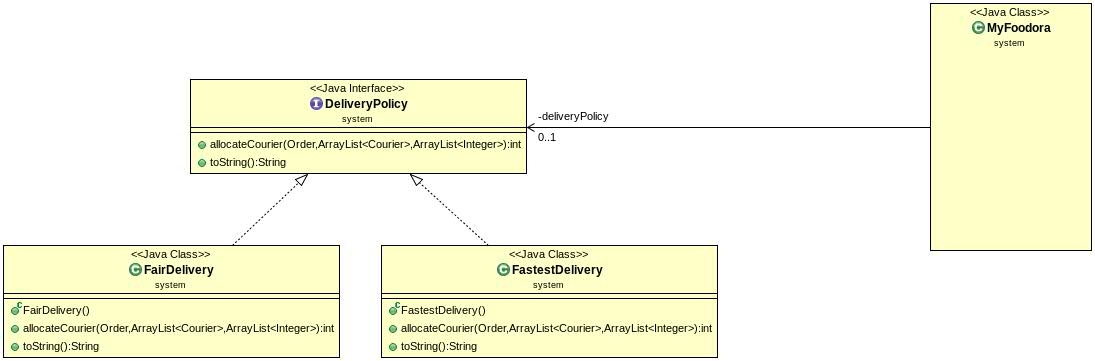
\includegraphics[width=0.8\linewidth]{./ima/deliverypolicy.jpg}
	\caption{Delivery Policy}
	\label{fig:deliveryPolicy}
\end{figure}


